Rozważania dotyczące PML zacznijmy od przypomnienia ogólnej postaci równania falowego
\begin{equation}
\nabla \cdot ( a \nabla U) = \frac{a}{b} \frac{\partial^2 u}{\partial t^2} = \frac{\ddot{u}}{b},
\end{equation}
gdzie przez $u(\vec{x},t)$ oznaczono skalarną amplitudę fali,a  $c=\sqrt{ab}$ jest prędkością fazową fali opisywanej powyższym równaniem dla dla parametrów $a(\vec{x})$,$b(\vec{x}$ opsiujących ośrodek, w którym zachodzi propagacja. Powyższe równanie różniczkowe drugiego rzędu, możemy zapisać w postaci dwóch równań z pierwszą pochodną poprzez wprowadzenie pola $\vec{v}(x,t)$:
\begin{equation}
\frac{\partial u}{\partial t} = b \nabla \cdot \vec{v},
\end{equation}

\begin{equation}
\frac{\partial \vec{v}}{\partial t}= a\nabla u.
\end{equation}
Bardziej abstrakcyjnie w postaci równania wektorowego powyższe dwa równania możemy zapisać jako
\begin{equation}
\frac{\partial \vec{w}}{\partial t}=\frac{\partial}{\partial t} {u \choose \vec{v}} = 
	\begin{pmatrix}
		& b\nabla\cdot \\
	a\nabla & \\
	\end{pmatrix}
{u \choose \vec{v}} = \hat{D}\vec{w},
\label{eq:gen-wave-eq}
\end{equation}
dla liniowego operatora $\hat{D}$ i czterowektora $\vec{w}=(u;\vec{v})$ ( w przestrzeni trójwymiarowej). Kluczową własnością, która decyduje o tym, że równanie \ref{eq:gen-wave-eq} jest ,,równaniem falowy'' okazuje się być antyhermitowskość operatora $\hat{D}$. To właśnie z tej własności wynikają oscylujące rozwiązania równania, spełnienie prawa zachowania energii, a przez to wszystkie zajwiska, które kojarzymy z fizyką fal. Każde równanie falowe, zaczynając od równań skalarnych, przez równania fali elektromagnetycznej po równanie Schr\"{o}dinger'a~(mechanika kwantowa) i równania Lam\'{e}-Navier'a~(fale sprężyste w ciałach stałych) mogą zostać przedstawione w formie $ \frac{\partial  \vec{w}}{\partial t}=\hat{D}\vec{w}$, dla pewnej funkcji falowej $\vec{w}$ i antyhermitowskiego operatora $\hat{D}$~\cite{johnson2007notes}. W niniejsze pracy skupiamy się na zastosowaniu PML w elektromagnetizmie, te same koncepcje mogą być jednak zastosowane do wszystkich wymienianych przypadków.

Załóżmy, że $w(x,t)$ jest rozwiązaniem równania falowego w nieograniczonej przestrzeni. Interesujące nas zjawiska zachodzą w okolicy początku układu współżędnych $x=0$, a obszar symulacji chcemy zakończyć tak aby absorbował fale propagujące się. W szczególności skupimy się na zakończeniu obszaru symulacji dla dodatniej części osi $+x$ (rozważanie dla pozostałych kierunków jest analogiczne). Zakończenie obszaru symulacji przeprowadzimy w trzech krokach:
\begin{enumerate}
	\item W nieskończonej przestrzeni wykonamy analityczne przedłużenie równania falowego i rozwiązania do zespolonego konturu $x$. Takie rozszerzenie zmienia fale propagujące się poza interesującym nas obszarem  fale zanikające bez wprowadzenia odbicia.
	\item Ciągle w nieograniczonej przestrzeni dokonamy zamiany współrzędnych, tak aby wyrazić zespolony $x$ przez rzeczywiste położenie. W nowych współrzędnych otrzymamy rzeczywiste położenia i materiały których własności są opisywane przy pomocy liczb zespolonych.
	\item Zakończymy obszar symulacji w obliczonym na podstawie zamiany zmiennych materiale w miejscu w którym pole będzie na tyle stłumione, aby zastosowany warunek brzegowy nie miał znaczenia.
\end{enumerate}

Zakładamy dalej, że przestrzeni znajdującej się daleko od interesującego nas obszaru w okolicach $x=0$ jest jednorodna, liniowa i niezmienia się w zależności od czasu. Dzięki tym założeniom fala propagująca się musi przyjmować formę superpozycji fal płaskich:
\begin{equation}
	w(\vec{x},t)= \sum_{\vec{k},\omega} W_{\vec{k},\omega} e^{i (kx-\omega t)},
\end{equation}
gdzie $W_{\vec{k},\omega}$ są stałymi amplitudami, $\omega$ częstością kołową, a $\vec{k}$ wektorem falowym (W ośrodku izotromowym związanymi zależnością dyspersyjną $\omega=c|\vec{k}|$, gdzie $c$ oznacza prędkość fazową). Dla fal propagujących się w kierunku $+x$ prędkość grupowa $\frac{d \omega}{d k}$ jest dodatnia. Kierunek prędkości fazowej i grupowej w ośrodkach jednorodnych są zgodne z wykluczeniem kilku szczególnych przypadków~\cite{teixeira1998general}. Dlatego dalej założymy, że $k$ jest dodatnie. 

\begin{figure}[tb]
	\begin{subfigure}{0.45\textwidth}
		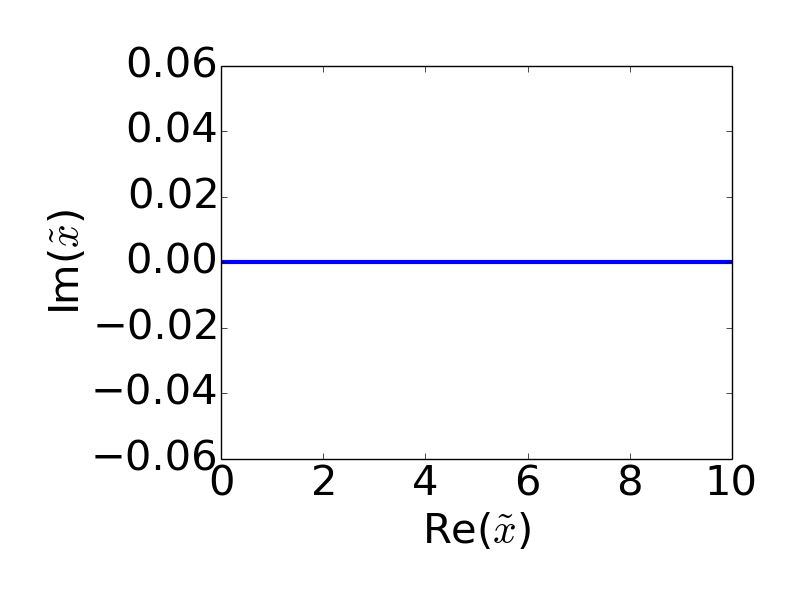
\includegraphics[width=\textwidth]{images/pml/real-x.png}
		\caption{}
	\end{subfigure}
	\begin{subfigure}{0.45\textwidth}
		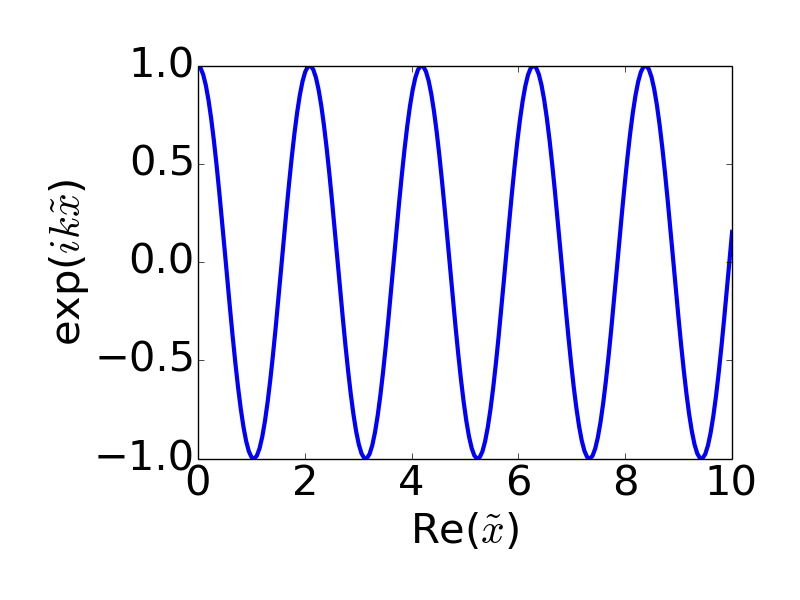
\includegraphics[width=\textwidth]{images/pml/real-x-wave.png}
		\caption{}
	\end{subfigure}


	\begin{subfigure}{0.45\textwidth}
		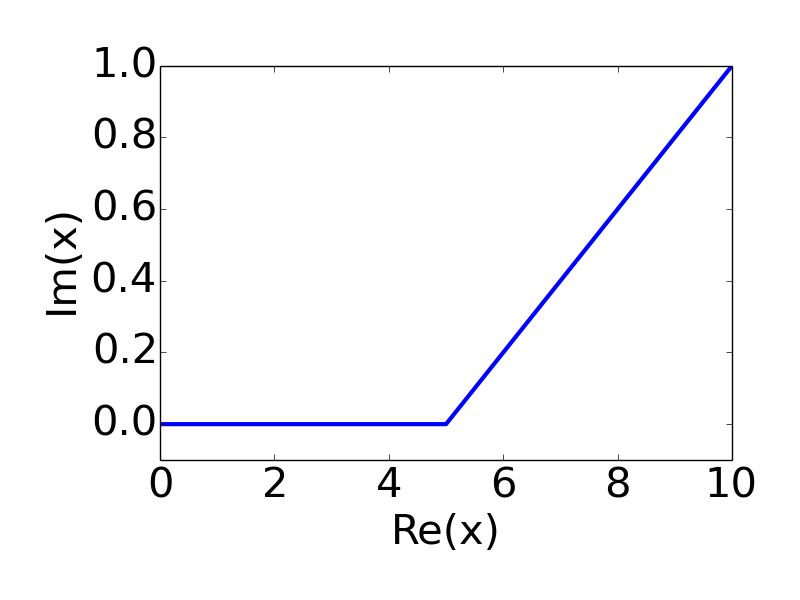
\includegraphics[width=\textwidth]{images/pml/complex-x.png}
		\caption{}
		\label{fig:complex-contour}
	\end{subfigure}
	\begin{subfigure}{0.45\textwidth}
		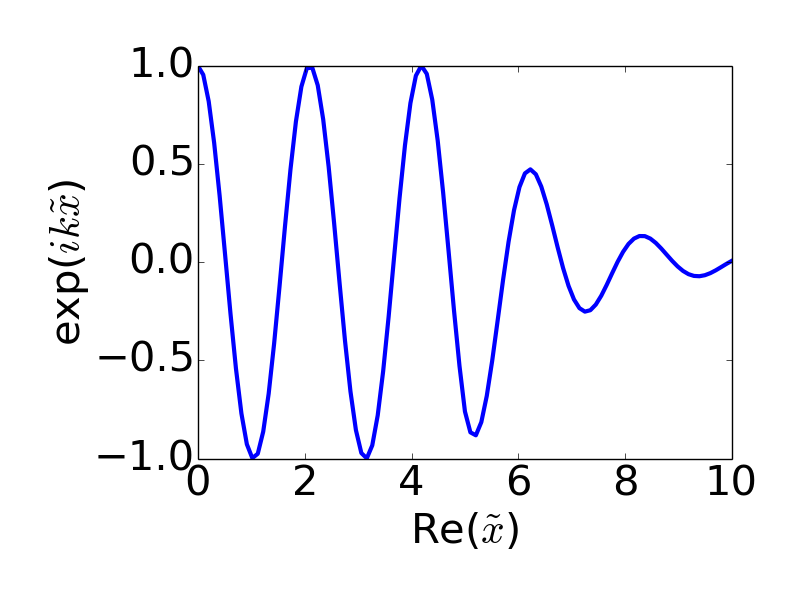
\includegraphics[width=\textwidth]{images/pml/complex-x-wave.png}
		\caption{}
		\label{fig:absorbing-region}
	\end{subfigure}

	\caption{Na rysunkach (a) i (b) odpowiednio przedstawiono rzeczywiste wartości położenia na zespolonej płaszczyźnie $x$ i odpowiadające im rozwiąanie równania falowego. Na rysunkach (c) dla wartości $x>5$ zasotoswano zmieniony kontur wyorzystujący zespolone wartości dla $x$, odpowiednie rozwiązanie równania falowego przedstawia wykres na rysunku (d).}
	\label{fig:var-transform}
\end{figure}


Kluczowym jest, że rozwiązania mogą zostać rozłożone w bazie funkcji postaci
\begin{equation}
\vec{W}(y,z)e^{i(kx-\omega t)},
\end{equation}
która to jest funkcją analityczną w x. Oznacza to, że możemy dokonać jej analitycznego przedłużenia dla zespolonych wartości $x$. Pierwotny problem fali propagującej się przedstawiają górne wykresy na rysunku \ref{fig:var-transform}. Jeżeli jednak zamiast rozważać propagację wzdłuż rzeczywistego $x$, rozwiążemy problem propagacji po zespolonym konturze przedstawionym na wykresie \ref{fig:complex-contour} zauważymy że dla obszaru w którym do rzeczywistej części dodaliśmy liniowo rosnącą część urojoną uzyskujemy falę zanikającą. Ponieważ na wykresie \ref{fig:absorbing-region} rozwiązanie dla $x<5$ nie uległo zmianie, a w obszarze $x>5$ obserwujemy fale zanikającą to przestrzeń dla $x>5$ wykazuje działanie nieodbijającej warstwy absorpcyjnej.

Dla wygody obliczeniowej przy stosowaniu tak powstałej warstwy zamiast stosować rozwinięcie analityczne możemy dokonać zamiany współrzędnych w omawianym równaniu różniczkowym. Oznaczmy zespolony $x$ przez $\tilde{x}(x)=x+if(x)$, traktując od tej pory $x$ zawsze jako rzeczywiste położenie. Taka zamiana współrzędnych wymaga od nas zamiany każdego różniczkowania po zdeformowanym konturze $\partial \tilde{x} = (1+i\frac{df}{dx}) \partial x$. Ponieważ założyliśmy, że nasze równanie różniczkowe jest niezależne od x (przynajmniej dla dużych x, gdzie $f(x)\ne0$) nie musimy uwzględniać żadnych dodatkowych wyrazów. Jak wykażemy w kolejnych akapitach wygodnie jest wybrać $\frac{df}{dx}=\frac{sigma_x}{\omega}$ i ostatecznie zapisać wymaganą zamianę zmiennych jako:
\begin{equation}
	\frac{\partial}{\partial x} \to \frac{1} {1+i \frac{\sigma_x(x)}{\omega}} \frac{\partial}{\partial x}.
	\label{eq:pml-variable-change}
\end{equation}

W obszarach PML, gdzie $\sigma_x\ne0$, oscylujące rozwiązania równania falowego przyjmują postać fal eksponencjalnie zanikających. Poza PML ( $sigma_x=0$) rozwiązywane równanie pozostaje niezmienione: nie występują odbicia ponieważ jest to analityczne rozwinięcie pierwotnego rozwiązania i w obszarach gdzie $\tilde{x}=x$ rozwiązanie nie może się zmienić.

Po wykonaniu podstawienia (\ref{eq:pml-variable-change}) rozwiązania równania falowego w obszarze PML przyjmują postać:
\begin{equation}
e^{ikx}e^{-\frac{k}{\omega}\int^x \sigma_x(x')dx'},
\end{equation}
warto zauważyć, że pojawiający się wykładnik potęgi $\frac{k}{\omega}$ dla materiałów bezdyspersyjnych jest stały i równy odwrotności prędkości fazowej. W ten sposób uzasadaniliśmy zaproponowany wybór $\frac{df}{dx}=\frac{\sigma_x}{\omega}$, dzięki któremu otrzymujemy niezależność współczynnika tłumienia od czętotliwości promieniowania E-M. 

Zasadniczo zgodnie z przedstawionym wyprowadzeniem możemy zastosować dowolnie mały obszar PML, ponieważ nie ma rzadnego ograniczenia na wartości $\sigma_x$. W praktyce numerycznej, ze względu na zastosowaną dyskretyzację gwałtowne zmiany $\sigma_x$ prowadzą do powstania ,,odbić numerycznych''. Z tego powodu $\sigma_x$ zazwyczaj ma postać funkcji kwadratowej lub sześćiennej narastającej od zera na obszarze większym od połowy długości fali promieniowania występującego w symulacji~\cite{johnson2008notes}.

W przypadku równań Maxwella każda zamiana współrzędnych może zostać wyrażona przez równania Maxwella we współrzędnych kartezjańskich ze zmienionymi materiałami~\cite{ward1996refraction}. Zamiana współrzędnych jest równoważna zmiane przenikalności elektrycznej $\varepsilon$ i magnetycznej $\mu$ w ogólności na absorbujące ośrodki anizotropowe. 

W ogólności w przypadku trójwymiarowych równań Maxwella dla ośrodka opisywanego przy pomocy tensorów $\hat{\varepsilon}$ i $\hat{\mu}$ 
\begin{equation}
\hat{\varepsilon}=
\begin{bmatrix}
\varepsilon_x & 0 & 0 \\
0 &\varepsilon_y & 0 \\
0 & 0  & \varepsilon_z  \\
\end{bmatrix}
, \hat{\mu}=
\begin{bmatrix}
\mu_x & 0 & 0 \\
0 &\mu_y & 0 \\
0 & 0  & \mu_z  \\
\end{bmatrix}
\end{equation}

warstwą PML może być materiał o charakteryzujący się przenikalnością elektryczną i magentyczną opisywaną ternsorami:
\begin{equation}
\hat{\varepsilon_{\textrm{PML}}}=
\begin{bmatrix}
s \cdot \varepsilon_x & 0 & 0 \\
0 &s \cdot \varepsilon_y & 0 \\
0 & 0  & \frac{ \varepsilon_z}{s}  \\
\end{bmatrix}
, \hat{\mu_{\textrm{PML}}}=
\begin{bmatrix}
s \cdot \mu_x & 0 & 0 \\
0 & s \cdot \mu_y & 0 \\
0 & 0  & \frac{\mu_z}{s}  \\
\end{bmatrix},
\label{eq:general-pml-form}
\end{equation}
gdzie $s$ jest dowolną liczbą zespoloną~\cite{sacks1995perfectly}, której część odpowiedzialna za tłumienie jest równoznaczna liniowemu współczynnikowi deformacji konturu zmiennych przestrzennych w część urojoną.


